



\chapter{Word Embeddings}

\section{Why vectors?}
We would like to have a structure 
\begin{enumerate}
    \item that can be modelled using a small(<- this depends on what your idea of small is, but we would like to have a memory efficient approach) number of parameters
    \item that has an inbuilt idea of similarity
    \item that can be easily manipulated
\end{enumerate}
As it turns out finite dimensional vector spaces are perfect for this task: the number of parameters is the number of dimensions, a metric can be used as notion of similarity, and we already have tools to manipulate them.





\section{Data Preparation}
We need to prepare the data or the next two models. We select a window size $n$. From the corpus, $n$ consecutive words are sampled. The middle word is the target word and the rest is the context. Each such target word, context pair is a data point.



\section{One-hot Representation of Words and Context}

Once the data preparation is done we will have a set of data points of the form $(S,W)$ where $S$ is the context and $W$ is the word. If the word is in the $i^{th}$ place in the vocabulary $V$ then we represent $W$ the one-hot vector $e_i$ ($i^{th}$ element of the standard basis). If the context contains the words $W_1=V[\alpha_1], W_2=V[\alpha_2]\hdots W_n=V[\alpha_n]$ then we will represent the context $S$ as $\sum_{i=1}^ne_{\alpha_i}$, i.e. the sum of the one-hot encoding of the individual words. For the rest of this discussion I will use the notation $w_i,V[i]$ and $e_i$ interchangeably for words. 








\section{Continuous bag of words model(CBOW)}
Assume we have a data point(we have taken size 5 for the example, but this should be adjusted as needed) as follows:
\begin{center}
    \textcolor{red}{Word1 Word 2} Word \textcolor{red}{Word3 Word 4}
\end{center} 
We model a classification problem where given context $\{$Word1, Word2, Word3, Word4$\}$ we wish to classify which word this set provides context for.[Note, when we represent it as a set, we automatically let go the notion of a sequence- hence the name 'bag of words']. For this we shall use a feed forward network described below:
\begin{enumerate}
    \item \textbf{Input :}For context $S\subset V$, we make an input vector $v$ where:
    $$v_S=\sum_{w_i\in S}e_i$$
    \item  \textbf{Hidden Layer 1}: This is obtained by multiplying $v$ by a matrix $W$. We denote:
    $$h_S=Wv_S$$
    For a single word $w_i$, $h_i=We_i=i^{th}$ column of $W$ will represent the hidden representation of $w_i$. 
    Therefore, if our context contains is $S=\{w_{\alpha_1},w_{\alpha_2},w_{\alpha_3},w_{\alpha_4}\hdots w_{\alpha_n}\}$ then our hidden representation of the context will be $h_S=W\left(\sum_{k=1}^n e_{\alpha_k}\right)=\sum_{k=1}^n h_{w_{\alpha_k}}$ (Note how our choice of using a linear space as structure of choice and setting the context as the linear combination of its constituents comes handy here)
    \item \textbf{Hidden Layer 2}: We use another matrix $W'$ and get
    $$y=W'h_S$$
    \item \textbf{Hidden Layer 3}: This is just a soft max to normalize things:
    $$\hat y=\text{Softmax}(y)$$
\end{enumerate} 
We use cross-entropy as our loss function of choice to train the model. $\hat y$ is compared to the one-hot representation of the word.

\begin{figure}
    \begin{center}
        

\tikzset{every picture/.style={line width=0.75pt}} %set default line width to 0.75pt        

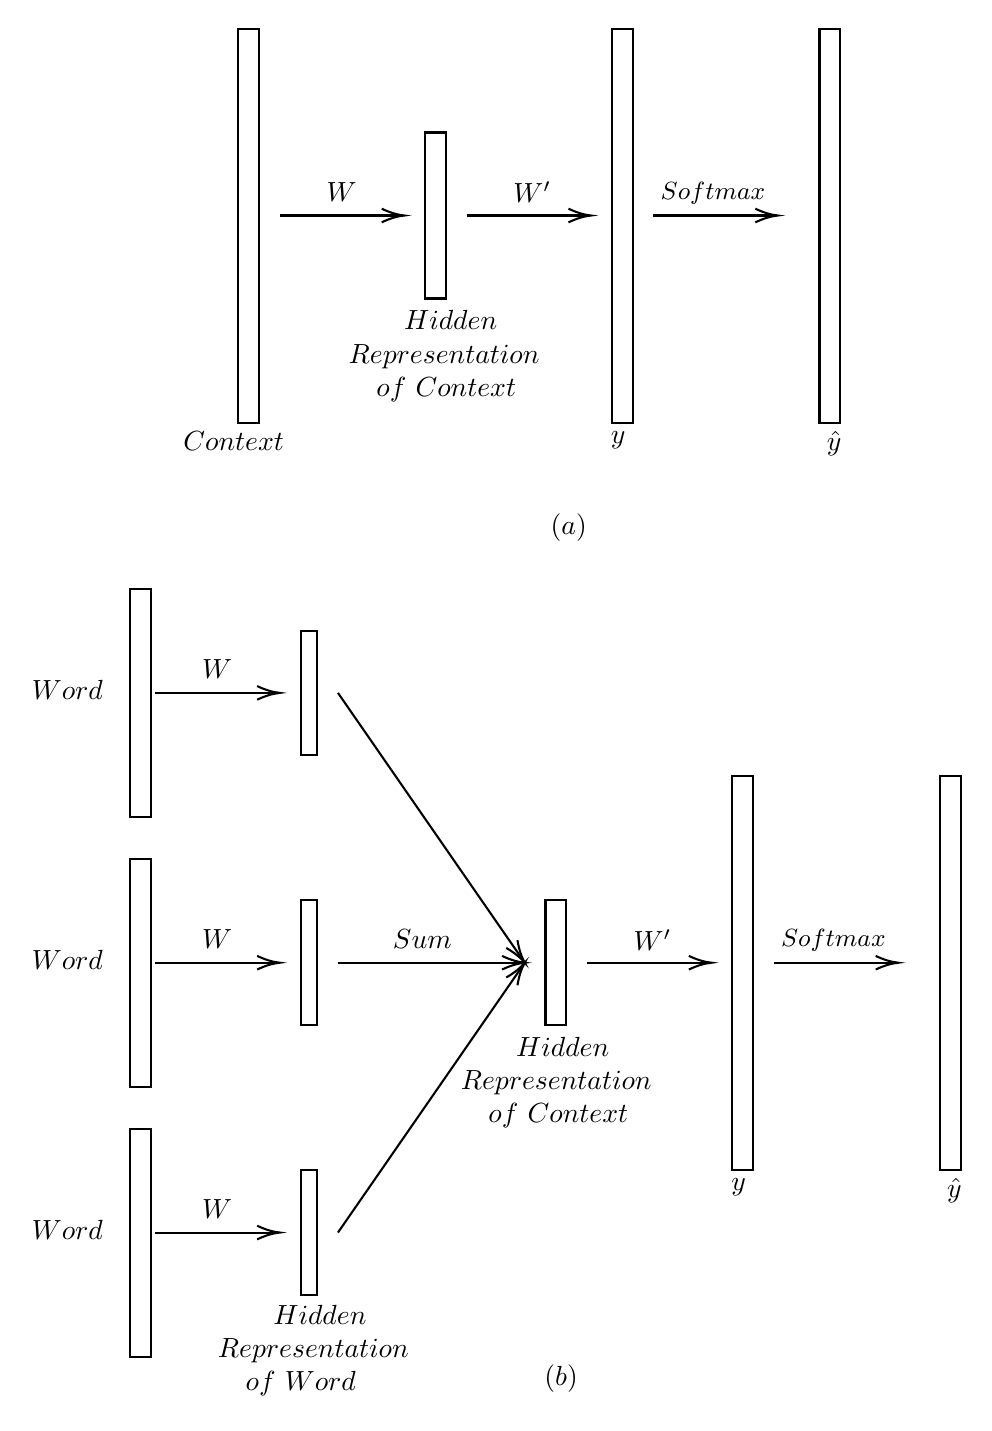
\begin{tikzpicture}[x=0.75pt,y=0.75pt,yscale=-1,xscale=1]
%uncomment if require: \path (0,744); %set diagram left start at 0, and has height of 744

%Shape: Rectangle [id:dp026521693413700476] 
\draw   (172,20) -- (182,20) -- (182,210) -- (172,210) -- cycle ;
%Straight Lines [id:da6320135821235765] 
\draw    (192,110) -- (250,110) ;
\draw [shift={(252,110)}, rotate = 180] [color={rgb, 255:red, 0; green, 0; blue, 0 }  ][line width=0.75]    (10.93,-3.29) .. controls (6.95,-1.4) and (3.31,-0.3) .. (0,0) .. controls (3.31,0.3) and (6.95,1.4) .. (10.93,3.29)   ;
%Shape: Rectangle [id:dp12692840020505802] 
\draw   (262,70) -- (272,70) -- (272,150) -- (262,150) -- cycle ;
%Straight Lines [id:da7459277485193251] 
\draw    (282,110) -- (340,110) ;
\draw [shift={(342,110)}, rotate = 180] [color={rgb, 255:red, 0; green, 0; blue, 0 }  ][line width=0.75]    (10.93,-3.29) .. controls (6.95,-1.4) and (3.31,-0.3) .. (0,0) .. controls (3.31,0.3) and (6.95,1.4) .. (10.93,3.29)   ;
%Shape: Rectangle [id:dp07310081517407963] 
\draw   (352,20) -- (362,20) -- (362,210) -- (352,210) -- cycle ;
%Straight Lines [id:da06986407926721172] 
\draw    (372,110) -- (430,110) ;
\draw [shift={(432,110)}, rotate = 180] [color={rgb, 255:red, 0; green, 0; blue, 0 }  ][line width=0.75]    (10.93,-3.29) .. controls (6.95,-1.4) and (3.31,-0.3) .. (0,0) .. controls (3.31,0.3) and (6.95,1.4) .. (10.93,3.29)   ;
%Shape: Rectangle [id:dp04257972028230528] 
\draw   (452,20) -- (462,20) -- (462,210) -- (452,210) -- cycle ;
%Shape: Rectangle [id:dp9098181133670411] 
\draw   (120,290) -- (130,290) -- (130,400) -- (120,400) -- cycle ;
%Straight Lines [id:da16252267787659302] 
\draw    (132,340) -- (190,340) ;
\draw [shift={(192,340)}, rotate = 180] [color={rgb, 255:red, 0; green, 0; blue, 0 }  ][line width=0.75]    (10.93,-3.29) .. controls (6.95,-1.4) and (3.31,-0.3) .. (0,0) .. controls (3.31,0.3) and (6.95,1.4) .. (10.93,3.29)   ;
%Shape: Rectangle [id:dp7664434843570327] 
\draw   (202,310) -- (210,310) -- (210,370) -- (202,370) -- cycle ;
%Straight Lines [id:da575597764045124] 
\draw    (340,470) -- (398,470) ;
\draw [shift={(400,470)}, rotate = 180] [color={rgb, 255:red, 0; green, 0; blue, 0 }  ][line width=0.75]    (10.93,-3.29) .. controls (6.95,-1.4) and (3.31,-0.3) .. (0,0) .. controls (3.31,0.3) and (6.95,1.4) .. (10.93,3.29)   ;
%Shape: Rectangle [id:dp7323495271401276] 
\draw   (410,380) -- (420,380) -- (420,570) -- (410,570) -- cycle ;
%Straight Lines [id:da16269082378611044] 
\draw    (430,470) -- (488,470) ;
\draw [shift={(490,470)}, rotate = 180] [color={rgb, 255:red, 0; green, 0; blue, 0 }  ][line width=0.75]    (10.93,-3.29) .. controls (6.95,-1.4) and (3.31,-0.3) .. (0,0) .. controls (3.31,0.3) and (6.95,1.4) .. (10.93,3.29)   ;
%Shape: Rectangle [id:dp33808841681535384] 
\draw   (510,380) -- (520,380) -- (520,570) -- (510,570) -- cycle ;
%Shape: Rectangle [id:dp7307300567221867] 
\draw   (120,420) -- (130,420) -- (130,530) -- (120,530) -- cycle ;
%Straight Lines [id:da39746393944318226] 
\draw    (132,470) -- (190,470) ;
\draw [shift={(192,470)}, rotate = 180] [color={rgb, 255:red, 0; green, 0; blue, 0 }  ][line width=0.75]    (10.93,-3.29) .. controls (6.95,-1.4) and (3.31,-0.3) .. (0,0) .. controls (3.31,0.3) and (6.95,1.4) .. (10.93,3.29)   ;
%Shape: Rectangle [id:dp6685146380753737] 
\draw   (202,440) -- (210,440) -- (210,500) -- (202,500) -- cycle ;
%Shape: Rectangle [id:dp40808635862127074] 
\draw   (120,550) -- (130,550) -- (130,660) -- (120,660) -- cycle ;
%Straight Lines [id:da5587676126883278] 
\draw    (132,600) -- (190,600) ;
\draw [shift={(192,600)}, rotate = 180] [color={rgb, 255:red, 0; green, 0; blue, 0 }  ][line width=0.75]    (10.93,-3.29) .. controls (6.95,-1.4) and (3.31,-0.3) .. (0,0) .. controls (3.31,0.3) and (6.95,1.4) .. (10.93,3.29)   ;
%Shape: Rectangle [id:dp6700192839775068] 
\draw   (202,570) -- (210,570) -- (210,630) -- (202,630) -- cycle ;
%Shape: Rectangle [id:dp8434692403820858] 
\draw   (320,440) -- (330,440) -- (330,500) -- (320,500) -- cycle ;
%Straight Lines [id:da7635704939549399] 
\draw    (220,340) -- (308.86,468.36) ;
\draw [shift={(310,470)}, rotate = 235.3] [color={rgb, 255:red, 0; green, 0; blue, 0 }  ][line width=0.75]    (10.93,-3.29) .. controls (6.95,-1.4) and (3.31,-0.3) .. (0,0) .. controls (3.31,0.3) and (6.95,1.4) .. (10.93,3.29)   ;
%Straight Lines [id:da1717667506724866] 
\draw    (220,600) -- (308.86,471.64) ;
\draw [shift={(310,470)}, rotate = 124.7] [color={rgb, 255:red, 0; green, 0; blue, 0 }  ][line width=0.75]    (10.93,-3.29) .. controls (6.95,-1.4) and (3.31,-0.3) .. (0,0) .. controls (3.31,0.3) and (6.95,1.4) .. (10.93,3.29)   ;
%Straight Lines [id:da6154675184222768] 
\draw    (220,470) -- (308,470) ;
\draw [shift={(310,470)}, rotate = 180] [color={rgb, 255:red, 0; green, 0; blue, 0 }  ][line width=0.75]    (10.93,-3.29) .. controls (6.95,-1.4) and (3.31,-0.3) .. (0,0) .. controls (3.31,0.3) and (6.95,1.4) .. (10.93,3.29)   ;

% Text Node
\draw (213,92.4) node [anchor=north west][inner sep=0.75pt]    {$W$};
% Text Node
\draw (303,92.4) node [anchor=north west][inner sep=0.75pt]    {$W'$};
% Text Node
\draw (374,92.4) node [anchor=north west][inner sep=0.75pt]  [font=\small]  {$Softmax$};
% Text Node
\draw (144,212.4) node [anchor=north west][inner sep=0.75pt]    {$Context$};
% Text Node
\draw (217,152.4) node [anchor=north west][inner sep=0.75pt]    {$ \begin{array}{l}
\ \ \ \ \ \ Hidden\\
Representation\\
\ \ \ of\ Context
\end{array}$};
% Text Node
\draw (350,212.4) node [anchor=north west][inner sep=0.75pt]    {$y$};
% Text Node
\draw (454,212.4) node [anchor=north west][inner sep=0.75pt]    {$\hat y$};
% Text Node
\draw (321,252.4) node [anchor=north west][inner sep=0.75pt]    {$( a)$};
% Text Node
\draw (153,322.4) node [anchor=north west][inner sep=0.75pt]    {$W$};
% Text Node
\draw (361,452.4) node [anchor=north west][inner sep=0.75pt]    {$W'$};
% Text Node
\draw (432,452.4) node [anchor=north west][inner sep=0.75pt]  [font=\small]  {$Softmax$};
% Text Node
\draw (408,572.4) node [anchor=north west][inner sep=0.75pt]    {$y$};
% Text Node
\draw (512,572.4) node [anchor=north west][inner sep=0.75pt]    {$\hat y$};
% Text Node
\draw (71,332.4) node [anchor=north west][inner sep=0.75pt]    {$Word$};
% Text Node
\draw (153,452.4) node [anchor=north west][inner sep=0.75pt]    {$W$};
% Text Node
\draw (71,462.4) node [anchor=north west][inner sep=0.75pt]    {$Word$};
% Text Node
\draw (153,582.4) node [anchor=north west][inner sep=0.75pt]    {$W$};
% Text Node
\draw (71,592.4) node [anchor=north west][inner sep=0.75pt]    {$Word$};
% Text Node
\draw (245,452.4) node [anchor=north west][inner sep=0.75pt]    {$Sum$};
% Text Node
\draw (271,502.4) node [anchor=north west][inner sep=0.75pt]    {$ \begin{array}{l}
\ \ \ \ \ \ Hidden\\
Representation\\
\ \ \ of\ Context
\end{array}$};
% Text Node
\draw (318,662.4) node [anchor=north west][inner sep=0.75pt]    {$( b)$};
% Text Node
\draw (154,631.4) node [anchor=north west][inner sep=0.75pt]    {$ \begin{array}{l}
\ \ \ \ \ \ Hidden\\
Representation\\
\ \ \ of\ Word
\end{array}$};


\end{tikzpicture}
\caption{Equivalent expression of CBOW}
    \end{center}
\end{figure}
We have:
$$\hat y=Softmax(W'(h_S))$$
But as $h_S$ is independent of all $h_{w}$ where $w\notin S$. Therefore, we don't compute $Wv_s$ nor do we keep track of all the weights. We look only at those columns of $W$ that correspond to words in the context and don't care about the rest. 
\subsection{Interpretation on a two word window}
Assume we have a two word window. We use a data point $(w_\alpha,w_\beta)$. Note that:
$$\mathcal{L}(w_\beta)=-\log \hat y_\beta=-\log\left(\frac{e^{y_\beta}}{\sum_{r} e^{y_r}}\right)$$
We do back propagation and calculate the gradients:
\begin{align*}
    \frac{\partial \mathcal L}{\partial y_i}=\hat y_i-\delta(i,\beta)
\end{align*}
Denote this as $E_i$ and define $E=[E_1, E_2\hdots E_n]$. Note $E=\hat y-$Observed $y$
\begin{align*}
    \frac{\partial \mathcal L}{\partial h_i}=\sum_{j}\frac{\partial \mathcal L}{\partial y_j}\frac{\partial y_j}{\partial h_i}= \sum_j E_j\frac{\partial \sum_k h_k W'_{k,j}}{\partial h_i}=\sum_j E_jW'_{ij}
\end{align*}
Therefore the gradient with respect to $h$ is
$$\nabla \mathcal L=W'^TE$$
This gives the update rules for $h$ as 
$$h:=h-\eta\nabla \mathcal L=h- \eta W\hat y+\eta W\text{ Observed }y$$
Assume  initial entries of $W$ to be small. Then and therefore, entries of $h_{Cat}$ and $h_{Dog}$ will have similar starting values: almost 0. Look at the following sentences:
\begin{center}
    Cat \textcolor{red}{sleeps}\\
    Dog \textcolor{red}{sleeps}
\end{center}
Note in both those cases, Observed $y$ will be same and therefore $h_{cat}$ and $h_{dog}$ will be adjusted in the same direction when they appear in similar context. This idea makes sure that similar words will have similar cosine similarity due to a form of transitive action. 

\section{Skip-Gram}
Skip-gram in a sense is CBOW trained in opposite direction. In this case we use a word to classify what context it comes from. The structure of the model is almost same as before.
\begin{figure}[h]
    \begin{center}
        

\tikzset{every picture/.style={line width=0.75pt}} %set default line width to 0.75pt        

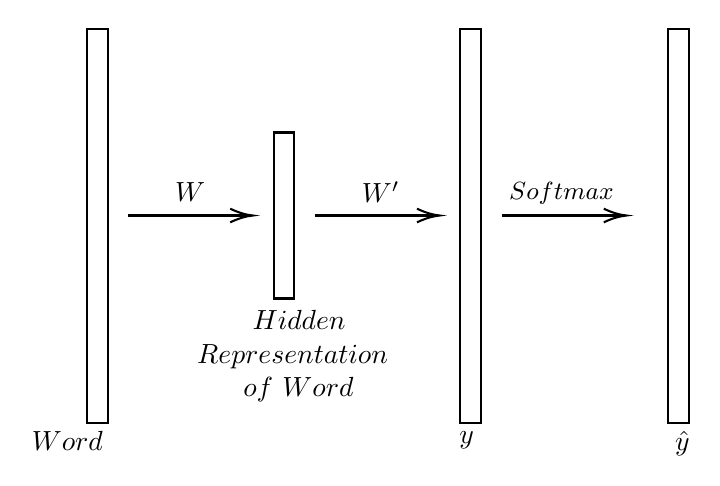
\begin{tikzpicture}[x=0.75pt,y=0.75pt,yscale=-1,xscale=1]
%uncomment if require: \path (0,300); %set diagram left start at 0, and has height of 300

%Shape: Rectangle [id:dp8690317092107768] 
\draw   (192,31) -- (202,31) -- (202,221) -- (192,221) -- cycle ;
%Straight Lines [id:da3129031681625205] 
\draw    (212,121) -- (270,121) ;
\draw [shift={(272,121)}, rotate = 180] [color={rgb, 255:red, 0; green, 0; blue, 0 }  ][line width=0.75]    (10.93,-3.29) .. controls (6.95,-1.4) and (3.31,-0.3) .. (0,0) .. controls (3.31,0.3) and (6.95,1.4) .. (10.93,3.29)   ;
%Shape: Rectangle [id:dp7964817410089358] 
\draw   (282,81) -- (292,81) -- (292,161) -- (282,161) -- cycle ;
%Straight Lines [id:da5578177280290412] 
\draw    (302,121) -- (360,121) ;
\draw [shift={(362,121)}, rotate = 180] [color={rgb, 255:red, 0; green, 0; blue, 0 }  ][line width=0.75]    (10.93,-3.29) .. controls (6.95,-1.4) and (3.31,-0.3) .. (0,0) .. controls (3.31,0.3) and (6.95,1.4) .. (10.93,3.29)   ;
%Shape: Rectangle [id:dp9023443845481357] 
\draw   (372,31) -- (382,31) -- (382,221) -- (372,221) -- cycle ;
%Straight Lines [id:da6062319286919925] 
\draw    (392,121) -- (450,121) ;
\draw [shift={(452,121)}, rotate = 180] [color={rgb, 255:red, 0; green, 0; blue, 0 }  ][line width=0.75]    (10.93,-3.29) .. controls (6.95,-1.4) and (3.31,-0.3) .. (0,0) .. controls (3.31,0.3) and (6.95,1.4) .. (10.93,3.29)   ;
%Shape: Rectangle [id:dp2886304505568057] 
\draw   (472,31) -- (482,31) -- (482,221) -- (472,221) -- cycle ;

% Text Node
\draw (233,103.4) node [anchor=north west][inner sep=0.75pt]    {$W$};
% Text Node
\draw (323,103.4) node [anchor=north west][inner sep=0.75pt]    {$W'$};
% Text Node
\draw (394,103.4) node [anchor=north west][inner sep=0.75pt]  [font=\small]  {$Softmax$};
% Text Node
\draw (164,223.4) node [anchor=north west][inner sep=0.75pt]    {$Word$};
% Text Node
\draw (237,163.4) node [anchor=north west][inner sep=0.75pt]    {$ \begin{array}{l}
\ \ \ \ \ \ Hidden\\
Representation\\
\ \ \ \ \ of\ Word
\end{array}$};
% Text Node
\draw (370,223.4) node [anchor=north west][inner sep=0.75pt]    {$y$};
% Text Node
\draw (474,223.4) node [anchor=north west][inner sep=0.75pt]    {$\hat{y}$};


\end{tikzpicture}

\caption{Schematic diagram of Skip gram}
    \end{center}
\end{figure}
\begin{enumerate}
    \item \textbf{Input :}For word $w_i$, the input is $v=e_i$
    \item  \textbf{Hidden Layer 1}: This is obtained by multiplying $v$ by a matrix $W$. We denote:
    $$h=Wv$$
    \item \textbf{Hidden Layer 2}: We use another matrix $W'$ and get
    $$y=W'h$$
    \item \textbf{Hidden Layer 3}: This is just a soft max to normalize things:
    $$\hat y=\text{Softmax}(y)$$
\end{enumerate}
The target output is  the one-hot representation of the context.
If we have a window size of $n$ our loss function, cross-entropy is the sum of $n-1$ terms. For example, if the data point has context $w_\alpha,w_\beta,w_\gamma,w_\delta$ then the loss function will be:
$$\mathcal L=- \log \hat y_\alpha- \log \hat y_\beta- \log \hat \hat y_\gamma- \log \hat y_\delta$$
Note that gradients are summed. For each term, the update to $h$ is the same as the one for CBOW. We again note that only the $i^{th}$ column of $W$ is updated: therefore we need not keep track of the rest of the weights. The interpretation of CBOW is carried over, this time with multi-word windows. For the sentences:
\begin{center}
    \textcolor{red}{My pet} Cat \textcolor{red}{sleeps}\\
    \textcolor{red}{My pet} Dog \textcolor{red}{sleeps}
\end{center}
Since both gives the same Observed $y$, $h_{Cat}$ and $h_{Dog}$ are adjusted in same direction, making them similar. 

\section{Negative sampling}
To improve performance, we might further want to make sure that words which are not similar are further apart. This gives rise to the idea of negative sampling. We make randomized context-word pairs which don't occur in the corpus. Therefore, we have two sets: $D=\{(S,W)\in Corpus\},D'=\{(S,W)\notin Corpus\}$. Define a random variable $Z$ as:
$$Z=\sigma\left(\hat y_{S}^T\cdot W\right)\text{ or }\sigma\left({S}^T\cdot \hat y_{W}\right)$$
We would like to maximize:
$$P(Z=1|(S,W)\in D)$$
$$P(Z=0|(S,W)\in D')$$
We use now compute the log-likelihood function as follows:\\
$\begin{aligned} & \underset{\theta}{\operatorname{maximize}} \prod_{(w, c) \in D} p(z=1 \mid w, c) \prod_{(w, r) \in D^{\prime}} p(z=0 \mid w, r) \\ & =\underset{\theta}{\operatorname{maximize}} \prod_{(w, c) \in D} p(z=1 \mid w, c) \prod_{(w, r) \in D^{\prime}}(1-p(z=1 \mid w, r)) \\ & =\underset{\theta}{\operatorname{maximize}} \sum_{(w, c) \in D} \log p(z=1 \mid w, c) +\sum_{(w, r) \in D^{\prime}} \log (1-p(z=1 \mid w, r)) \\ & =\underset{\theta}{\operatorname{maximize}} \sum_{(w, c) \in D} \log \frac{1}{1+e^{-v_c^T v_w}}+\sum_{(w, r) \in D^{\prime}} \log \frac{1}{1+e^{v_r^T v_w}} \\ & =\underset{\theta}{\operatorname{maximize}} \sum_{(w, c) \in D} \log \sigma\left(v_c^T v_w\right)+\sum_{(w, r) \in D^{\prime}} \log \sigma\left(-v_r^T v_w\right) \\ & \end{aligned}$\\
This leads to a better loss function. Ideally we would want $k$ bad $w,s'$ pairs in $D'$ for each correct $w.s$ in $D$. Since the number of bad combinations is significantly more than the number of correct combinations, $k>1$, where $k$ is a hyperparameter to be tuned. The samples are picked from a modified unigram distribution with $p(r)\sim count(r)^{p}$. The original word2vec used $p=0.75$, but it can also be trained as a hyperparameter. Unless we properly tune $k$ and $p$, $SVD$ gives better performance. 
\section{Contrastive Estimation}
The problem is soft-max is expensive. So instead of using soft max, we give it a score.  Assume for elements of $D$ we get a total score of $s$ and for elements of $D'$ we get a total score of $s'$. We make our objective to maximise $max(0,s-s-m)$: We claim that if the difference is $m$, then we are happy with the contrast.







\section{SVD to learn word representations}
We consider two arrays: a corpus $C$ and a vocabulary $V$. We assume that the context of a word is given by words at a distance $d$ away from it. Define a co-occurance matrix $\mathcal M$ defined as:
$$\mathcal M[i][j]=\{\text{Number of occurrence of }w_i\text{ and }w_j\text{ with distance at most }d\}$$
Consider the SVD decomposition of $\mathcal M$ as $\mathcal M=U\sum V$. Represent the columns of $U$ as $U_i$s and the rows of $V$ as $V_i^T$. The $k^{th}$ rank approximation of $\mathcal M$ is given by:
$$\hat{\mathcal M}_k=\sum_{i=1}^k \sigma_i U_iV_i^T $$
This representation brings out latent relations between variables. Now we define the representation  of the $i^{th}$ word as the $i^{th}$ row of $U\sum$. This reduces the size of representation while keeping the cosine similarity fixed.















\section{GloVe Representations}
We combine count based methods(like SVD) and Prediction based methods(CBOW, Skip gram). For words $V[i]$ and $V[j]$ we would like to have a representations $h_i,h_j$ that is faithful to $\mathcal M$ i.e:
$$h_i\cdot h_j =\log(j|i)=\log \mathcal M[i][j]-\log X_i$$
$$h_j\cdot h_i =\log(i|j)=\log \mathcal M[j][i]-\log X_j$$
Where $X_i,X_j$ are the counts of occurrences of $X_i$ and $X_j$
We combine to get:
$$h_i\cdot h_j=\mathcal{M}[i][j]-\frac{1}{2}\left(\log X_i+\log X_j\right)$$

But the problem with this is it weights all co-occurances equally. To circumvent this issue, We replace $X_i,X_j$ as trainable weights $b_i,b_j$. Therefore, our loss function becomes:
$$\sum_{w_i,w_j}\left(\mathcal M[i][j]-b_i-b_j-h_i\cdot h_j\right))$$ 















\section{Other embeddings}
Suppose we have some unstructured data with some underlying notion of similarity(For example: Faces, Words, Sentences, Graphs etc.). We can generalise the above-mentioned process of embeddings to get an alternate representation of such data in a low dimensional vector space while retaining their inherent notion of similarity.